\section{Обзор предметной области}
\subsection{Задача компьютерного зрения}
Компьютерное (машинное) зрение – это совокупность программно-технических решений в сфере искусственного интеллекта (ИИ), нацеленных на считывание и получение информации из изображений, в реальном времени и без участия человека. 

Большое количество информации человек получает при помощи зрения. 

В основе компьютерного зрения лежит 
В настоящий момент, такие технологии применяются для решения таких сложных задач как:
\begin{itemize}
    \item OCR – Optical character recognition (Оптическое распознавания символов): преобразование текста на изображении в редактируемый.
    \item Фотограмметрия – технология создания трехмерной модели объекта на основе фотографий, сделанных с различных ракурсов.
    \item Motion capture – технология, широко применяемая в киноиндустрии, позволяющая преобразовывать движения реальных людей в компьютерную анимацию.
    \item Дополненная реальность (AR) – технология, позволяющая в реальном времени проецировать виртуальные объекты на изображение реального окружения. 
    \item Медицинская диагностика – обнаружение раковых клеток на ранней стадии, увеличение качества МРТ изображений, их анализ и т.д.
\end{itemize}
\subsection{Искусственные нейронные сети}

\subsubsection{Понятие искусственной нейронной сети}

Машинное обучение – раздел исследований в сфере ИИ, в основе которых лежат методы разработки систем способных к обучению. ???

Искусственная нейронная сеть (ИНС) – компьютерная модель, в основе которой лежат принципы работы биологической нейронной сети - совокупности связанных между собой нервных клеток - нейронов. Каждый нейрон имеет набор входных связей - синапсов, по которым он получает информацию, представленную в виде импульсов, от других нейронов. По полученным данным нейрон формирует своё состояние и, с помощью аксона, сообщает его другим нейронам, обеспечивая функционирование системы. В процессе формирования системы одни нейронные связи укрепляются, а другие ослабляются, обеспечивая обучаемость сети.
\addimghere{biological-neuron}{0.5}{Типичная структура нейрона}{biological-neuron}
Искусственный нейрон представляет собой упрощенную модель биологического нейрона. На вход подаются n-мерные вектор значений $X=(x_{1},...,x_{n})$ и вектор весов $W=(w_{1},...,w_{n})$. Входные значения несут информацию, а веса указывают на "силу" межнейронных связей. Процесс подбора весов называется обучением нейронной сети. Значение выхода нейрона вычисляется по формуле: 
\[
  out(x)=\sigma(\sum_{\mathclap{i=1}}^{n} x_{i}w_{i})
\]
Где $\sigma$ - функция активации.

\subsubsection{Активационная функция}
При вычислении взвешенной суммы входов нейрона, результат может принимать абсолютно любое значение $x\in(-\infty;+\infty)$, что препятствует дальнейшим вычеслениям.
Активационная функция нейрона обеспечивает нормализацию посчитанной суммы, таким образом, что значение выхода нейрона всегда принадлежит некоторому, заранее заданному, диапазону, часто: $(0;1)$ или $(-1;1)$. Для многих моделей нейронных сетей также требуется, чтобы активационная функция была нелинейной, монотонной и непрерывно-дифференцируемой на всей области определения.

Существует большое количество функций активации. Наиболее распространенные из них представлены в табл. \ref{actvs}

\pgfplotsset{
  every axis plot/.append style={
    line width=3pt
  }
}

\begin{table}[H]
  \centering
  \caption{Популярные активационные функции}\label{actvs}
  \begin{tabular}{|c|c|c|}
    \hline    
    \hyperlink{name}{Название} & \hyperlink{func}{Функция} & \hyperlink{chart}{Вид}\\
    \hline
    Сигмоидная &  \resizebox{0.2\hsize}{!}{$\sigma(x)=\frac{1}{1+e^{-x}}$}
    & 
    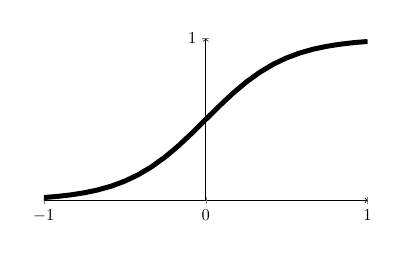
\begin{tikzpicture}[baseline={(0,0.8)}, scale=0.6]      
      \begin{axis}[
        axis equal image,
        axis lines=middle,
        axis line style={->},
        x label style={at={(axis description cs:0.5,-0.1)},anchor=north},
        y label style={at={(axis description cs:-0.1,.5)},rotate=90,      anchor=south},
        extra x ticks=0,
        % extra y ticks=1,
        ymin=0,ymax=1,
        ytick={0, 1},
        xtick={-1, 0, 1}
        ]
        \addplot[domain=-1:1, variable=\x] ({\x},{1/(1+exp(-4*\x))});
      \end{axis}      
    \end{tikzpicture}
   
    \\
    \hline
    Гиперболический тангенс 
    &
    \resizebox{0.2\hsize}{!}{$f(x)=\frac{e^x-e^{-x}}{e^x+e^{-x}}$}
    & 
    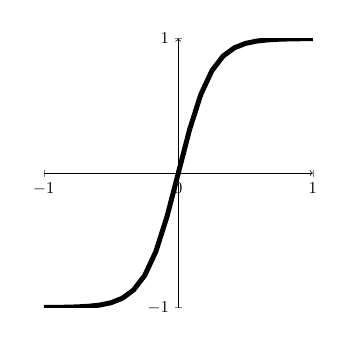
\begin{tikzpicture}[baseline={(0,1.5)},scale=0.6]
      \begin{axis}[
        axis equal image,
        axis lines=middle,
        axis line style={->},
        x label style={at={(axis description cs:0.5,-0.1)},anchor=north},
        y label style={at={(axis description cs:-0.1,.5)},rotate=90,      anchor=south},
         extra x ticks=0,  
        % extra y ticks=1,
        ymin=-1,ymax=1,
        ytick={-1, 0, 1},
        xtick={-1, 0, 1}
        ]
        \addplot[domain=-1:1, variable=\x]({\x},{tanh(4*\x)});
      \end{axis}      
    \end{tikzpicture} 
    \\
    \hline
    ReLU & \resizebox{0.2\hsize}{!}{$f(x) =\begin{cases}
    0, & x<0 \\ 
    x, & x \geq 0.
    \end{cases}$} & 
    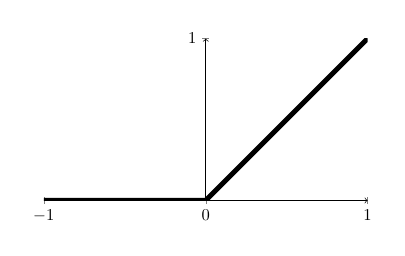
\begin{tikzpicture}[baseline={(0,0.8)},scale=0.6]
      \begin{axis}[
        axis equal image,
        axis lines=middle,
        axis line style={->},
        x label style={at={(axis description cs:0.5,-0.1)},anchor=north},
        y label style={at={(axis description cs:-0.1,.5)},rotate=90,anchor=south},
         extra x ticks=0,  
        % extra y ticks=1,
        ymin=0,ymax=1,
        ytick={0, 1},
        xtick={-1, 0, 1}
        ]
        \addplot[domain=-1:1, variable=\x]({\x},{ifthenelse(\x<0,0,\x)});
      \end{axis}      
    \end{tikzpicture}
    \\
    \hline
  \end{tabular}
\end{table}

\subsubsection{Структура нейронной сети}
Множества нейронов формируют слои, слои в свою очередь формируют нейронную сеть. Входной слой получает данные, обрабатывает и передает нейронам скрытого слоя. Аналогично срабатывет каждый последующий слой вплоть до выходного. 

\tikzset{%
every neuron/.style={
  circle,
  draw,
  minimum size=1cm
},
neuron missing/.style={
  draw=none, 
  scale=4,
  text height=0.333cm,
  execute at begin node=\color{black}$\vdots$
},
}
\begin{figure}[H]
  \centering
\begin{tikzpicture}[x=1.5cm, y=1.5cm, >=stealth]

\foreach \m/\l [count=\y] in {1,2,3,missing,4}
\node [every neuron/.try, neuron \m/.try] (input-\m) at (0,2.5-\y) {};

\foreach \m [count=\y] in {1,missing,2}
\node [every neuron/.try, neuron \m/.try ] (hidden-\m) at (2,2-\y*1.25) {};

\foreach \m [count=\y] in {1,missing,2}
\node [every neuron/.try, neuron \m/.try ] (output-\m) at (4,1.5-\y) {};

\foreach \l [count=\i] in {1,2,3,n}
\draw [<-] (input-\i) -- ++(-1,0)
  node [above, midway] {$I_\l$};

\foreach \l [count=\i] in {1,k}
\node [above] at (hidden-\i.north) {$H_\l$};

\foreach \l [count=\i] in {1,p}
\draw [->] (output-\i) -- ++(1,0)
  node [above, midway] {$O_\l$};

\foreach \i in {1,...,4}
\foreach \j in {1,...,2}
  \draw [->] (input-\i) -- (hidden-\j);

\foreach \i in {1,...,2}
\foreach \j in {1,...,2}
  \draw [->] (hidden-\i) -- (output-\j);

\foreach \l [count=\x from 0] in {Входной, Скрытый, Выходной}
\node [align=center, above] at (\x*2,2) {\l \\ слой};
\end{tikzpicture}
\caption{Схема простой нейронной сети} \label{simple-network}
\end{figure}
\subsubsection{Глубокие нейронные сети}
Под глубокими нейронными сетями понимают сети с большим количеством скрытых слоев.
\subsubsection{Сверточные нейронные сети}
???
\subsubsection{Проблемы обучения нейронных сетей}
???
\subsection{Применение нейронных сетей в задачах распознавания изображений}
???
\clearpage